% This is the start of every LaTeX document. The document class specifes the overall type of
% document you are writing. 'article' is most common. 'report' is similar to 'article', but allows
% for chapters. 'book' is for writin large books. 'beamer' for making presentations
\documentclass{article}

% Below are all the included packages. Packages add extra functionality to default LaTeX by adding
% new macros or changing default behaviours
\usepackage[margin=35mm]{geometry} % Controls layout of the page, including margins
\usepackage{biblatex}              % Controls bibliography and citations
\usepackage{listings}              % Source code layout, formatting and styling
\usepackage{color}                 % Needed for coloring source code syntax
\usepackage[hidelinks]{hyperref}   % Support for links. Autolinks citations, references, and TOC
\usepackage{amsmath}               % Maths equations and aligns
\usepackage{amssymb}               % More maths symbols
\usepackage{graphicx}              % For including images
\usepackage{subcaption}            % For using subfigures
\usepackage{booktabs}              % For prettier looking tables and better rules

% Sets the title and author of the document. This is printed by \maketitle
% If date is not specified with \date{}, the current date is used
\title{\LaTeX{} Workshop}
\author{Tim Quelch}

% Add the references to the bibliography
\addbibresource{references.bib}

% Style options for souce code blocks (listing environment, and \lstinline{} macro)
\lstset{
	language=TeX,              % Language for syntax highlighting
	basicstyle=\ttfamily,      % Style for fonts
	numbers=left,              % Line numbers
	numberstyle=\tiny,         % Line number style
	frame=tb,                  % Frame lines on top and bottom
	tabsize=4,                 % Size of tabs
	columns=fixed,             % Fix character columns
	showstringspaces=false,    % Don't underscore spaces
	showtabs=false,            % Don't underscore tabs
	keepspaces,                % Keep spaces as spaces, not whitespace
	commentstyle=\color{red},  % Colour comments as red
	% keywordstyle=\color{blue},% Colour keywords as blue
	breaklines=true,           % Break lines, so they don't go over the page
}

% TODO config section numbers
% TODO config font selection
% TODO config fancy header

% All the actual content of the document goes in the document environment
\begin{document}

% Prints the title, author, and date.
\maketitle

% Prints the table of contents generated from the sections
\tableofcontents

% Inserts a page break (new page)
\newpage

\section{Introduction}
``\LaTeX{} is a high-quality typesetting system; it includes features designed for the production of technical and scientific documentation. \LaTeX{} is the de facto standard for the communication and publication of scientific documents. \LaTeX{} is available as free software.''
\cite{latex_project_latex_2018},

One of the key differences in \LaTeX{} to more common work processors (MS Word, LibreOffice etc.) is the separation of content and presentation. In \LaTeX{} the author describes the general structure of the document (section headings, paragraphs, equations, figures), and the layout and typesetting is handled by \LaTeX{} (or rather the underlying \TeX{} backend).

There are several advantages to this:
\begin{itemize}
  \item Author can focus on the actual content, rather than making everything look pretty
  \item Presentation can be changed easily without major formatting reworks throughout the document
  \item A standard(ish) format for submission to external publishers, who can then apply their own layout/presentation styles
\end{itemize}

\LaTeX{} is written in plain text, and is processed by an external program to generate the output files (usually a PDF)

\subsection{Pronounciation and Spelling}
\LaTeX{} is always \emph{lah-tech}, and sometimes \emph{lay-tech}. It is never pronounced \emph{lay-tecks}. It is always written with the \lstinline|\LaTeX{}| macro (output is the weird sized and spaced \LaTeX{}), or with the capitialistaion LaTeX.

\subsection{Language Structures}
There are two major language structures that you will encounter when using \LaTeX{}: macros, and environments.

Macros are how we tell \LaTeX{} to do things. They take the general form of \lstinline{\commandname}, or with arguments \lstinline|\commandname[optional args]{required args}|. Macros can do anything from printing the table of contents (\lstinline{\tableofcontents}), \emph{emphasising} or \textbf{bolding} text (\lstinline|\emph{emphasising},\textbf{bolding}|), or even printing the funny \LaTeX{} logo (\lstinline|\LaTeX{}|). It is even possible to define your own macros to simplify things you are repeating often.

Environments are how we write larger sections of the document which often contain many lines or macros. Environments begin with a \lstinline|\begin{environmentname}| macro, and end with a \lstinline|\end{environmenname}| macro. Common environments include \lstinline{figure}, \lstinline{equation}, \lstinline{itemize} (these will be discussed later).

\subsection{The Preamble}
The preamble contains all the configuration and setup before the actual content.

The first line of the preamble is setting the \lstinline{\documentclass}. This tells \LaTeX{} what kind of document you are writing. The most common one used is \lstinline{article}. Other ones include \lstinline{report} which is similar to \lstinline{article}, but allows for chapters. \lstinline{book} is for writin large books. You can even write powerpoint presentations with the \lstinline{beamer} class.

The preamble also includes all the package inclusions for the document with the \lstinline|\usepackage{packagename}| macro. Packages add extra functionality to default \LaTeX{} by adding new macros or changing default behaviours. For example, the \lstinline{amsmath} package adds support for more maths environments and symbols, \lstinline{graphicx} allows for the inclusion of image files for figures.

Any extra configuration for styling and layout is also done in the preamble.

\subsection{\lstinline{document} Environment}
All of the actual content of the document goes in the \lstinline{document} environment

% TODO Preamble document environment

\section{Useful structure things} % TODO rename?

\subsection{Sections}
Sections are used to divide the document into parts. A new section is started with the \lstinline|\section{sectionname}| macro. Section titles are formatted to be bigger, bolded, and automatically numbered.

The table of contents (\lstinline{\tableofcontents}) is generated from the section headings. All the page numbers and section numbers are set automatically.

\subsection{Subsections}
We can also split sections into smaller \lstinline|\subsections{subsectionname}|
\subsubsection{Subsubsection}
... and \lstinline|\subsubsections{subsubsectionname}|

\subsection*{Unnumbered sections}
Sections and subsections can be unnumbered if they are declared with an asterisk. e.g.\ \lstinline|\section*{section name}|. The current subsection is un numbered in this way

% TODO

% TODO snippe to turn off all numbering

\subsection{Lists}
% TODO

Dot point lists are created with the \lstinline{itemize} environment
\begin{itemize}
  \item Each item begins with the \lstinline{\item} macro
  \item another item
  \item another item
    \begin{itemize}
      \item You can also do nested lists by just starting a new \lstinline{itemize} environment
        \begin{itemize}
          \item And the marker changes for each level you are on
            \begin{itemize}
              \item List markers and spacing and spacing can be customised with the \lstinline{enumitem} package
            \end{itemize}
        \end{itemize}
    \end{itemize}
\end{itemize}


Numbered lists are created with the \lstinline{enumerate} environment
\begin{enumerate}
  \item Each item begins with the \lstinline{\item} macro
  \item another item
  \item another item
    \begin{enumerate}
      \item You can also do nested lists by just starting a new \lstinline{enumerate} environment
        \begin{enumerate}
          \item And the marker changes for each level you are on
            \begin{enumerate}
              \item List markers and spacing and spacing can be customised with the \lstinline{enumitem} package
            \end{enumerate}
        \end{enumerate}
    \end{enumerate}
\end{enumerate}

\section{Maths}

% TODO aligns, equations,
% TODO Text, greek symbols

\href{https://www.rpi.edu/dept/arc/training/latex/LaTeX_symbols.pdf}{The Great, Big List of \LaTeX{} Symbols} \cite{carlisle_great_2001}

\begin{equation}
    \alpha \beta \gamma \delta \epsilon \varepsilon \zeta \eta \theta \vartheta \iota \kappa \lambda \mu \nu \xi \pi \varpi \rho \varrho \sigma \varsigma \tau \upsilon \phi \varphi \chi \psi \omega
\end{equation}
\begin{equation}
    \Gamma \Delta \Theta \Lambda \Xi \Pi \Sigma \Upsilon \Phi \Psi \Omega
\end{equation}
% TODO Proof environment

\section{Figures, Tables, and Code}

\begin{figure}[h!]
    \centering
    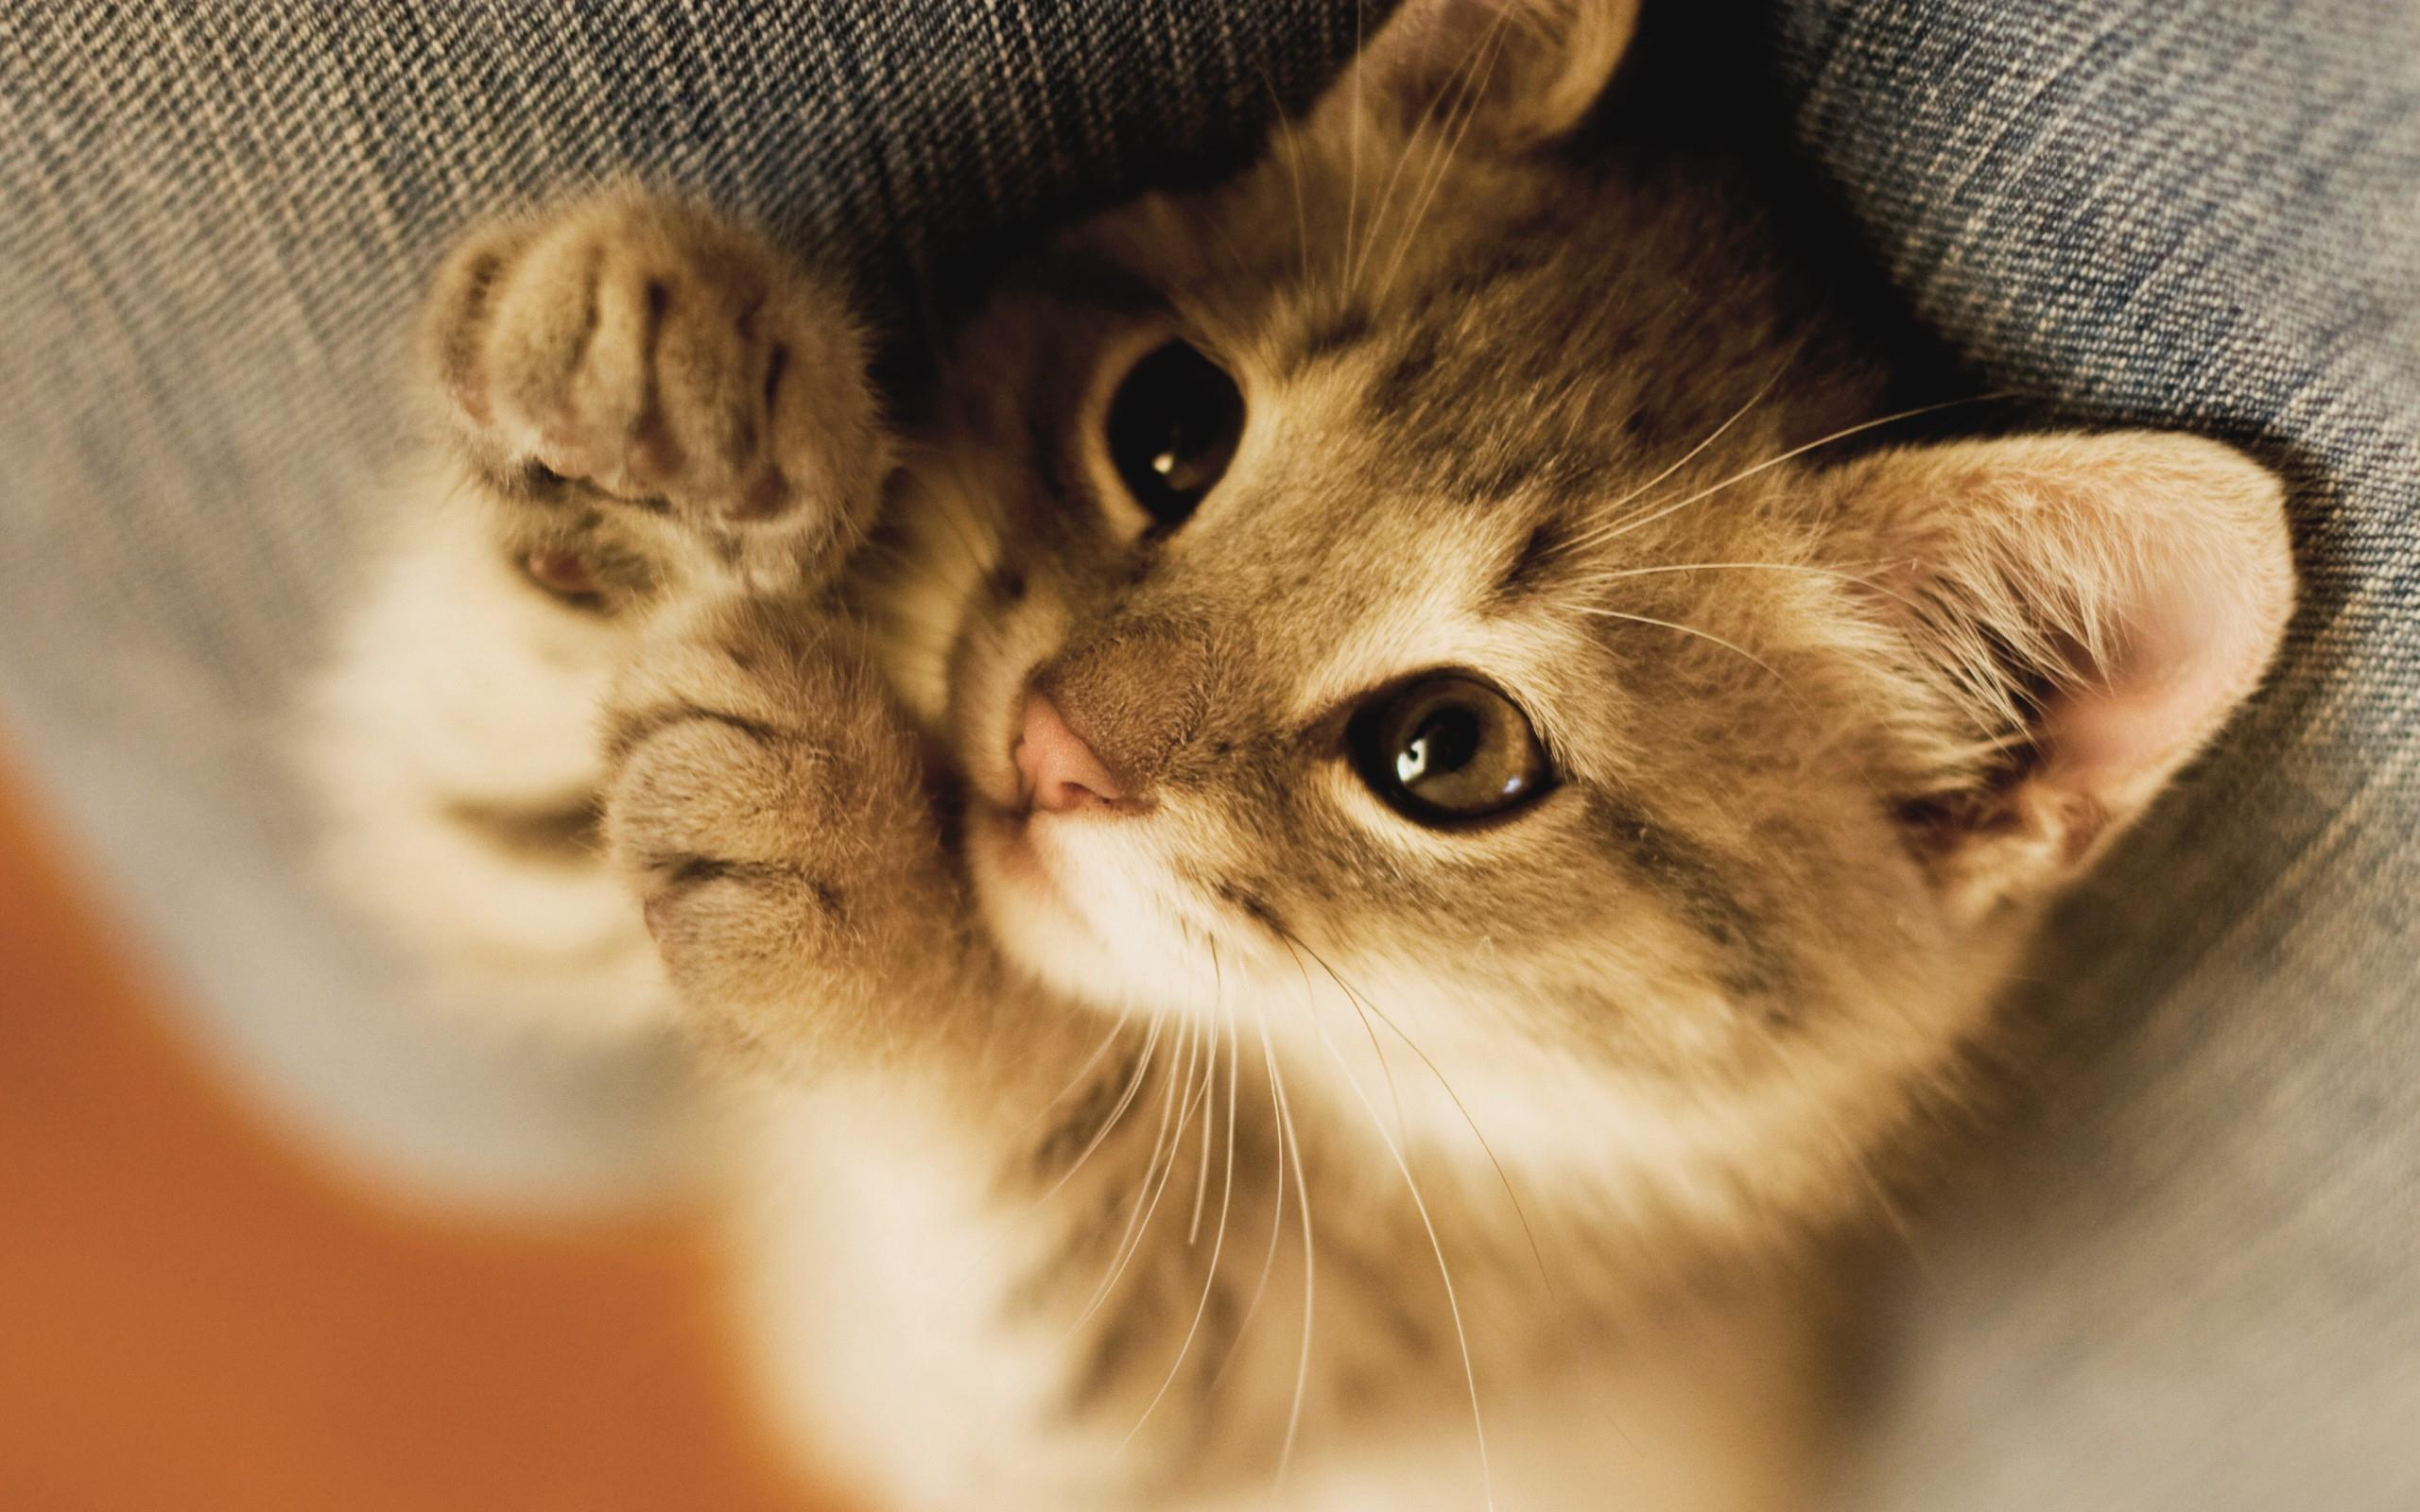
\includegraphics[width=0.7\textwidth]{cat.jpg}
    \caption{This is a caption for the figure. The figure numbering is automatic}
\end{figure}

\begin{figure}[h!]
    \centering
    \begin{subfigure}{0.47\textwidth}
        
\includegraphics[height=5.5cm]{rabbit.jpg}
        \caption{The first subfigure}
    \end{subfigure}
    ~
    \begin{subfigure}{0.47\textwidth}
        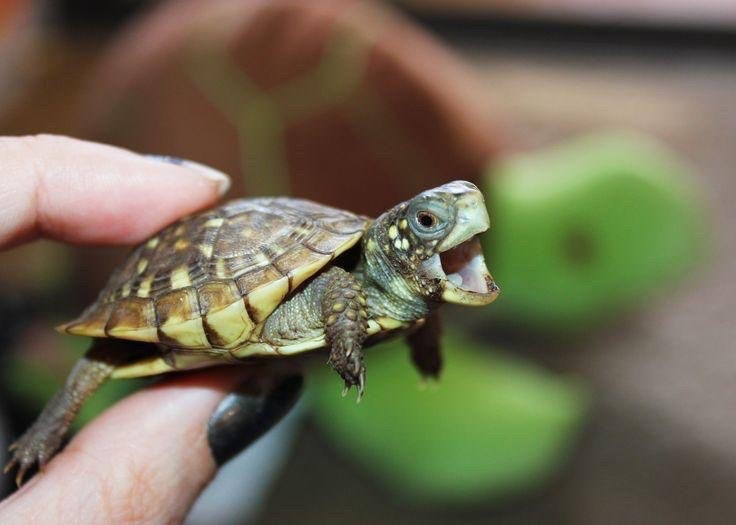
\includegraphics[height=5.5cm]{turtle.jpg}
        \caption{The second subfigure}
    \end{subfigure}
    \caption{A caption for both subfigures}
\end{figure}

\begin{table}
    \centering
    \caption{Caption for a table. This generally goes above the table}
    \begin{tabular}{lrr}
      \toprule
      & Column 1 & Column 2 \\
      \midrule
      Row 1 & 7 & 2 \\
      Row 2 & 8 & 9 \\
      Row 3 & 2 & 0 \\
      Row 4 & 4 & 1 \\
      \bottomrule
    \end{tabular}
\end{table}

\subsection{References \& Labels}

% TODO

\subsection{\LaTeX{} knows better than you}

% TODO

\subsection{Build your own}

% TODO

\section{Citations}

% TODO

\printbibliography

\end{document}